\section{Introduction}
\label{sec:intro}

\begin{figure}[t]
  \centering
  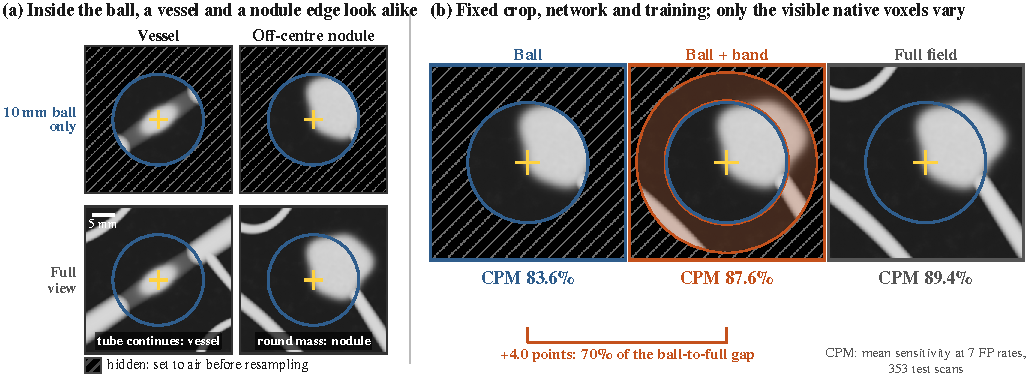
\includegraphics[width=\columnwidth]{figures/teaser.pdf}
  \caption{What a wider view adds at a fixed proposal. (a)~Inside the $10\mm$ ball, a vessel crossing the slice and the edge of an off-centre nodule look alike; the full view separates them. (b)~With crop, network and training fixed, restoring a thin band around the ball (hidden voxels hatched, set to air) raises CPM from \BallCpm\% to \BandCpm\%, closing \PrimaryRecovery\% of the gap to the full field. Synthetic phantom, to scale.}
  \label{fig:teaser}
\end{figure}

Pulmonary nodule detection in chest CT is commonly organized in two stages: a candidate generator proposes locations with high sensitivity, and a false-positive reduction network ranks the candidates so that true nodules precede false marks~\cite{setio2017luna16,setio2016multiview,dou2017multilevel}. Rankers that observe a wider field around each proposal perform better~\cite{dou2017multilevel,kim2018mgi}, yet the source of this improvement has received little attention. A wider field may reveal surrounding anatomy, for instance a vessel that continues beyond a bright cross-section, or it may simply reveal more of the lesion when the proposal is displaced from the nodule centre or the nodule exceeds the local view (Fig.~\ref{fig:teaser}a). Comparing patch sizes cannot distinguish these explanations, because a larger patch changes both at once.

In this work, we separate them with a controlled \emph{visibility intervention}. The proposal locations, the input tensor, the network and the training recipe are held fixed, and only the set of voxels of the original (\emph{native}) scan that the ranker may observe is varied: a $10\mm$ ball around the proposal (hereafter the \emph{ball}), the ball together with a thin spherical shell just outside it (hereafter the \emph{band}), or the full $32.4\mm$ crop (the \emph{full field}). We refer to the network trained on each condition as the ball-only, band and full-field ranker. Hidden voxels are set to air \emph{before} resampling, which guarantees that no hidden intensity reaches the input through interpolation (Fig.~\ref{fig:visibility}c), and every model is trained under the visibility with which it is evaluated.

On the \EvalScans{} LUNA16 evaluation scans, restoring the band raises the competition performance metric (CPM) of a two-scale 3D ranker from \BallCpm\% to \BandCpm\% ($+4.03$ points; $+4.21$ points for a second training seed), closing \PrimaryRecovery\% and \RepeatRecovery\% of the gap between the ball-only and the full-field ranker. Unlike multi-scale and nested-context rankers~\cite{dou2017multilevel,kim2018mgi}, which enlarge the input together with the architecture, and unlike occlusion analyses of trained networks~\cite{zeiler2014visualizing,fong2017meaningful}, which present masked inputs a model never saw during training, our intervention changes only the native evidence and retrains every model under the visibility it is evaluated with. This makes it possible to ask not only whether the extra field helps, but what in it does.

A simple geometric example shows why the answer is not obvious. Consider a spherical nodule whose centre is displaced from the proposal, and compute the fraction of its volume that falls inside the $10\mm$ ball and inside the band, which spans $10.3$--$15.0\mm$ for typical voxel spacings (Sec.~\ref{sec:band}; same geometry as Fig.~\ref{fig:teaser}). A $5\mm$ nodule displaced by $2\mm$ lies entirely inside the ball, so the band can only add surroundings. For a $14\mm$ nodule displaced by $6\mm$, the ball contains 78\% of the nodule and the band a further 18\%, and for a $20\mm$ nodule displaced by $8\mm$ the ball contains only 43\% while the band adds another 42\%. Whether a wider view contributes context or lesion therefore depends on lesion size and on how far the proposal is from the lesion centre, and an analysis of context must be able to tell the two apart.

Our paper offers the following contributions. First, we introduce a visibility intervention that changes only the native evidence available to a ranker, with masking before resampling so that hidden voxels cannot leak into the input (Sec.~\ref{sec:visibility}). Second, a coverage control shows that exposing the same image network only to the native voxels behind 384 sparse samples of the band recovers less than half of its gain (Sec.~\ref{sec:source_result}). Third, a geometry control shows that sparse readouts with direction-aware attention gain at most about one CPM point, far below the dense band (Sec.~\ref{sec:spatial_result}). Fourth, an anatomy-based analysis shows that the gains concentrate in the roughly one sixth of lesions whose annotated tissue the band reaches, as the example above predicts, with a consistent effect for a second 3D architecture (Secs.~\ref{sec:anatomy_result} and~\ref{sec:breadth_result}). Together, these results indicate that much of the benefit of wider context at fixed proposals comes from observing more of the lesion, with any contribution of the surrounding anatomy within the crop smaller and less certain.

\section{Related work}
\label{sec:related}

The LUNA16 challenge established a common candidate set and evaluation protocol for false-positive reduction, which made rankers directly comparable~\cite{setio2017luna16}. Multi-view 2D networks combine differently oriented planes~\cite{setio2016multiview}, and 3D networks with several receptive fields~\cite{dou2017multilevel}, nested fields of view~\cite{kim2018mgi} and end-to-end detectors~\cite{ding2017accurate,zhu2018deeplung,baumgartner2021nndetection,ardila2019endtoend} report that larger 3D context is beneficial. These works, however, vary the patch size, the number of streams or the architecture jointly, so the gain cannot be attributed to the additional evidence alone. Earlier hand-crafted methods made the role of the surroundings explicit: Hessian-based filters distinguish dot-like nodules from line-like vessels~\cite{li2003selective}, and spherical-shell features~\cite{leemput2015shell} and spectra of intensity profiles on spheres~\cite{ciompi2015frequencies} describe the neighbourhood of a candidate to separate vessels from nodules. These studies motivate our exterior band, but we use their sampling geometry to define what is made visible rather than as a feature, and we compare the sparse samples with the dense region that contains them while holding the network fixed.

Our analysis also relates to work on identifying the evidence a network relies on. Removing or masking parts of the input is a standard tool for this purpose~\cite{zeiler2014visualizing,fong2017meaningful}, but masking the input of a trained network produces inputs it has never seen, and retraining under the mask avoids this distribution shift~\cite{hooker2019benchmark}. We follow the retraining approach and train and evaluate every visibility condition under its own mask. Such analyses are particularly relevant in medical imaging, where networks can exploit unintended cues~\cite{geirhos2020shortcut,zech2018variable} and the effective receptive field may be considerably smaller than the nominal one~\cite{luo2016erf}. Finally, to read the sparse samples we build on permutation-invariant pooling~\cite{zaheer2017deep} and set attention~\cite{lee2019set,wang2018nonlocal}, adding a fixed bias that encodes the angle between sample directions in order to test whether the relative geometry of the samples, which a pooled readout discards, accounts for their lower performance.

\begin{figure}[t]
  \centering
  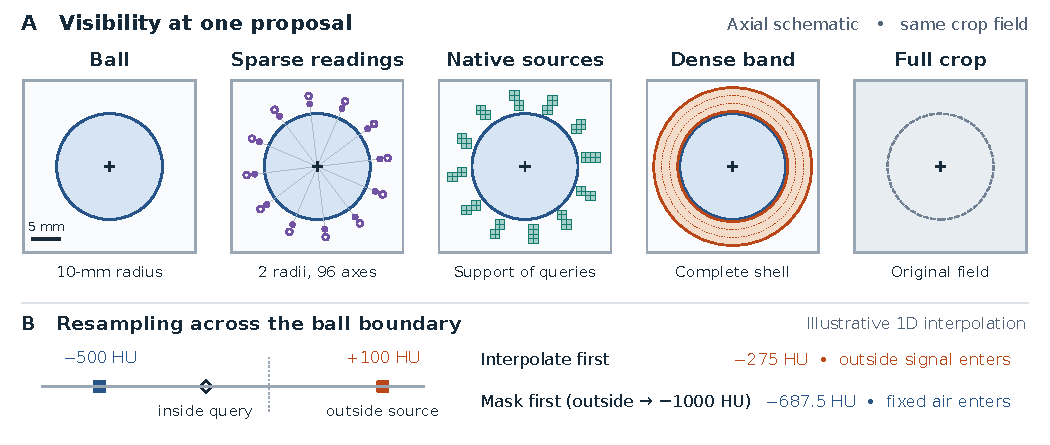
\includegraphics[width=\columnwidth]{figures/visibility.pdf}
  \caption{Visibility conditions at one proposal (cross). (a)~The four image conditions: ball $B(p)$, ball plus native sources $U(p)$, ball plus band $A(p)$, and full field; hidden voxels are hatched. (b)~The sparse samples on both ends of each axis at radii $r_N$ and $r_F$ (12 of 96 axes shown; created in BioRender, labels added). (c)~Masking before resampling admits only air from hidden voxels (Lemma~\ref{lem:leakage}).}
  \label{fig:visibility}
\end{figure}
